
Um robô autônomo móvel capaz de executar tarefas rotineiras domésticas pode ser dividido em diversas funcionalidades individuais que contém suas próprias dificuldades e desafios. Dentre elas, uma pode ser considerada elementar e é o foco deste trabalho: a navegação do robô. Ademais, na área da robótica móvel, se encontram diversas abordagens para o controle lógico do robô, a sua estrutura física e até a forma de locomoção dele. Com isso, este capítulo expõe os conhecimentos básicos sobre estes tópicos e a simulação do modelo do robô a ser proposto.


\section{Robô Autônomo Móvel} %%MANTER
Os robôs autônomos móveis são sistemas mecânicos com certo grau de inteligência,  capazes de transitarem em um meio com liberdade, lidarem com as possíveis mudanças na sua trajetória e executarem tarefas determinadas \cite{practicalIndroductionNehmzow:2012}. 

Os robôs autônomos móveis são constituídos por uma estrutura física, seu corpo, composta por elementos que possibilitam a sua percepção do meio que estão inseridos (sendo estes os sensores) e que executam ações diante do mesmo (denominados como atuadores) \cite{mobileRoboticsJaulin:2019}.
Para controlarem seu corpo, é implementado um sistema de controle inteligente que toma decisões a partir da interpretação dos dados coletados pelos sensores e essas decisões são enviadas aos atuadores para que a atividade em execução prossiga \cite{mobileRoboticsJaulin:2019}. 

Esses equipamentos são utilizados em diversas áreas, como medicina, agricultura e militarismo \cite{mobileRoboticsJaulin:2019}. 
Através deles, é possível executar tarefas comumente realizadas por algum ser vivo (como seres humanos ou animais) ou veículos, tais quais podem ser perigosas ou não desejáveis por uma determinada razão \cite{mathematicsModelsKelly:2013}.
Por poderem ser estruturas robustas,  permitem chegar a localizações que os seres humanos não conseguem acessar \cite{mobileRoboticsJaulin:2019}. 
Isso permite a execução de funcionalidades como: transportação, inspeção e segurança\cite{mobileRoboticsJaulin:2019}. 

Assim, os robôs móveis autônomos são vantajosos principalmente por definirem, praticarem e adaptarem um planejamento da execução de uma tarefa conforme o seu aprendizado do ambiente \cite{practicalIndroductionNehmzow:2012}. 
O diferencial entre os robôs móveis autônomos e outros robôs dependentes, é a sua adaptabilidade perante mudanças no ambiente e não conterem ações pré-definidas \cite{practicalIndroductionNehmzow:2012}.

Sendo assim, um dos maiores desafios encontrados na área é o tratamento e tomada de decisões do robô perante mudanças constantes em um ambiente interno com um alto grau de incerteza, como pessoas (sejam elas adultas, crianças ou idosos) e animais transitando, ademais do próprio  posicionamento de móveis e objetos \cite{practicalIndroductionNehmzow:2012}. 
 
Dito isso, esta seção apresenta os conceitos básicos de navegação, da estrutura física de um robô móvel autônomo e a discussão sobre as abordagens de arquiteturas mais relevantes para o seu controle lógico.


\subsection{Navegação Autônoma do Robô }

A navegação de um robô de forma independente não constitui apenas do dispositivo vagar pelo local aonde se encontra. Em primeiro lugar, é necessário que ele entenda onde está e com isso possa identificar o seu ponto geográfico no espaço em que atua. Em conjunto com a tarefa que deseja executar e as informações do ambiente, o robô inicia o processo de planejamento da trajetória que precisa percorrer até o seu destino. Por fim, a partir das decisões tomadas para seguir uma rota, ele se moverá inteligentemente até o destino, evitando os obstáculos e lidando com possíveis mudanças no meio. Assim, podemos afirmar que a navegação autônoma do robô é composta por quatro tarefas primordiais: i) percepção do ambiente, ii) localização, iii) planejamento, iv) locomoção \cite{mobileRobotsSiegwart:2011}. 

É necessário que o papel do robô e o seu ambiente de atuação sejam bem definidos. Desse modo, as funcionalidades essenciais afirmadas conseguem ser integradas, a fim de atender melhor os requisitos e manter a confiabilidade no dispositivo \cite{mobileRobotsSiegwart:2011}. 
Isso é notório ao comparar o funcionamento de um robô com um braço robótico que empilha paletes em uma fábrica em detrimento a um robô aspirador de pó — apesar de ambos serem robôs autônomos móveis.

Como explicitado, a primeira ação que um robô autônomo móvel deve executar antes de se mover por um ambiente, é a percepção do mesmo. Entender qual a situação atual do meio e as suas características, pode ser realizado por um conjunto de sensores que coletam dados ao redor do robô, como luminosidade, amplitude do som e medida da distância \cite{mobileRobotsSiegwart:2011}. 
Com o conhecimento adquirido através das informações processadas com os dados reunidos pelos sensores, é possível identificar o ponto geográfico onde o robô se encontra no espaço \cite{mobileRobotsSiegwart:2011}.

Com a percepção completa do ambiente, as informações registradas são utilizadas para localizar o robô no espaço. \citet{mobileRoboticsJaulin:2019} reconhece a localização como a identificação da posição do robô no ambiente e seu grau de liberdade para movimentação. Essa etapa é considerada um dos principais desafios da navegação, existindo diversas abordagens.

Entre as abordagens existentes para a localização, é mais comum o uso de modelos reais (como mapas topográficos), podendo ser criados dinamicamente enquanto o robô navega pelo ambiente ou ser uma entrada pré-definida do sistema \cite{mobileRobotsSiegwart:2011}. 
Por outro lado, esse método é questionado, pois, muitas vezes, o modelo não é verossímil à realidade. Para isso, são utilizadas técnicas alternativas como equações de matemática com ângulos e características cinemáticas de marcos ao redor do robô \cite{mobileRoboticsJaulin:2019}.

A localização do robô em um meio e o mapeamento desse ambiente é um problema bem conhecido na área da robótica móvel \cite{SLAMProblem:1991}. Uma das alternativas encontradas para ultrapassar essa questão são os algoritmos que implementam a abordagem SLAM (em inglês \textit{Simultaneous Localization and Mapping}). A abordagem de Mapeamento e Localização Simultânea tem o intuito de produzir um mapa consistente do ambiente, a partir de leituras de sensores ou câmeras, e obter a localização estimada do robô conforme os pontos reais encontrados no meio e os seus correspondentes no mapa criado \cite{SLAMDefinitionEvolution:2021, SLAMTutorialII:2006, SLAMReview:2015}. Uma das maiores vantagens encontradas na utilização do SLAM é a irrelevância da localização do robô e das informações do ambiente antes da sua execução \cite{SLAMReview:2015}.

Após compreender o ambiente e onde o robô se encontra, esse elabora um plano para seguir sua trajetória a fim de terminar a tarefa em execução.
Nesse contexto, surge outro problema significativo da navegação: a capacidade de chegar ao seu destino de forma eficiente e confiável \cite{mobileRobotsSiegwart:2011}.

Como apontam \citet{mobileRobotsSiegwart:2011}, um ponto crítico da tarefa de planejamento é a própria movimentação do robô. A cada “passo” que ele avança, as características do ambiente mudam, como, por exemplo, o robô pode estar chegando cada vez mais perto de uma parede que deve desviar em um futuro próximo. Dessa forma, o robô também atua no meio, intervindo nas suas características. 

Especificamente, ao tratar de um robô autônomo móvel que atua em um ambiente interno como um domicílio, a dificuldade aumenta, por ser um espaço dinâmico e vivenciado por seres humanos que são menos previsíveis do que objetos ou móveis parados. Portanto, é fundamental que a arquitetura do robô tenha um nível de inteligência suficiente para elaborar um caminho, evitando colisões, e o seu redirecionamento para longe dos obstáculos e mais próximo do destino.

Embora um planejamento sólido para navegação, considerando os aspectos de percepção e localização, seja de fundamental importância, a estratégia de locomoção adequada não pode ser deixada de lado. Segundo \citet{mobileRobotsSiegwart:2011}, existem duas principais maneiras de um robô se mover pelo espaço: uma forma veicular (por rodas) ou assemelhando-se a biologia (por pernas). 

O uso de rodas é comumente optado para robôs que atuam em terrenos mais regulares e lisos, visando um melhor desempenho. Neste contexto, a escolha da roda usada impacta a direcionalidade do robô. De um lado, há a roda comum (Figura~\ref{fig:rodas}(a)) que traz a necessidade de mudar o eixo do corpo para se locomover em outra direção e de outro, há rodas como a roda Mecanum (Figura~\ref{fig:rodas}(b)) que permite a mudança de direção sem a mudança no eixo. Além do seu design, a quantidade de rodas e a disposição delas impactam na estabilidade, controle e manobras do robô. 
 
\begin{figure}[h]
    \centering
    \caption{Diferença entre roda padrão e roda Mecanum}
    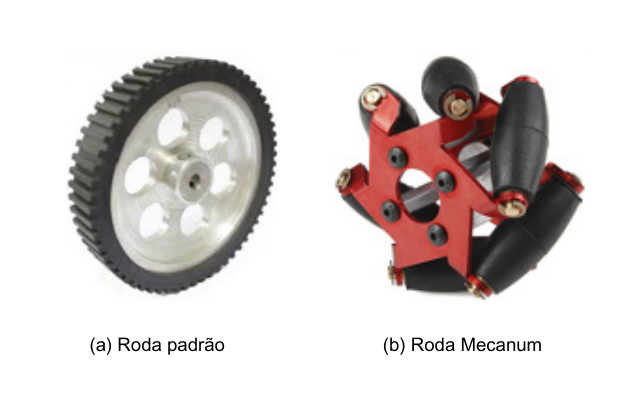
\includegraphics[scale=0.5]{rodas.png}
    \caption*{Fonte: \citet{wheels:2018}.}
    \label{fig:rodas}
\end{figure}

\subsection{Abordagens de Arquitetura de Controle} 

A navegação consegue ser bem sucedida apenas quando os seus quatro aspectos fundamentais (percepção, localização, planejamento e locomoção) são controlados corretamente de forma uníssona por uma arquitetura inteligente \cite{mobileRobotsSiegwart:2011}. Para isso, existem duas abordagens principais que possam ser utilizadas: hierarquica e comportamental. A principal diferença encontrada nessas abordagens é a sua organização interna para atingir o objetivo necessário.

As abordagens hierarquicas, como a inteligência artificial (IA) clássica, controlam o robô de forma sequencial. A estrutura dessa abordagem é constituída pelo processamento das informações do ambiente sequencialmente conforme o modelo do mundo real utilizado em cada camada da estrutura \cite{practicalIndroductionNehmzow:2012,toroco:2022}. Como pode ser visto na Figura~\ref{fig:iaclassica}, os dados captados pelos sensores alimentam a primeira funcionalidade da estrutura. Com isso, essa camada inicial executa seu próprio processamento e repassa os seus resultados para a próxima funcionalidade. Por fim, o resultado da última camada é inferida nos atuadores do robô para que este complete a sua atuação desejada.

\begin{figure}[h]
    \centering
    \caption{IA clássica}
    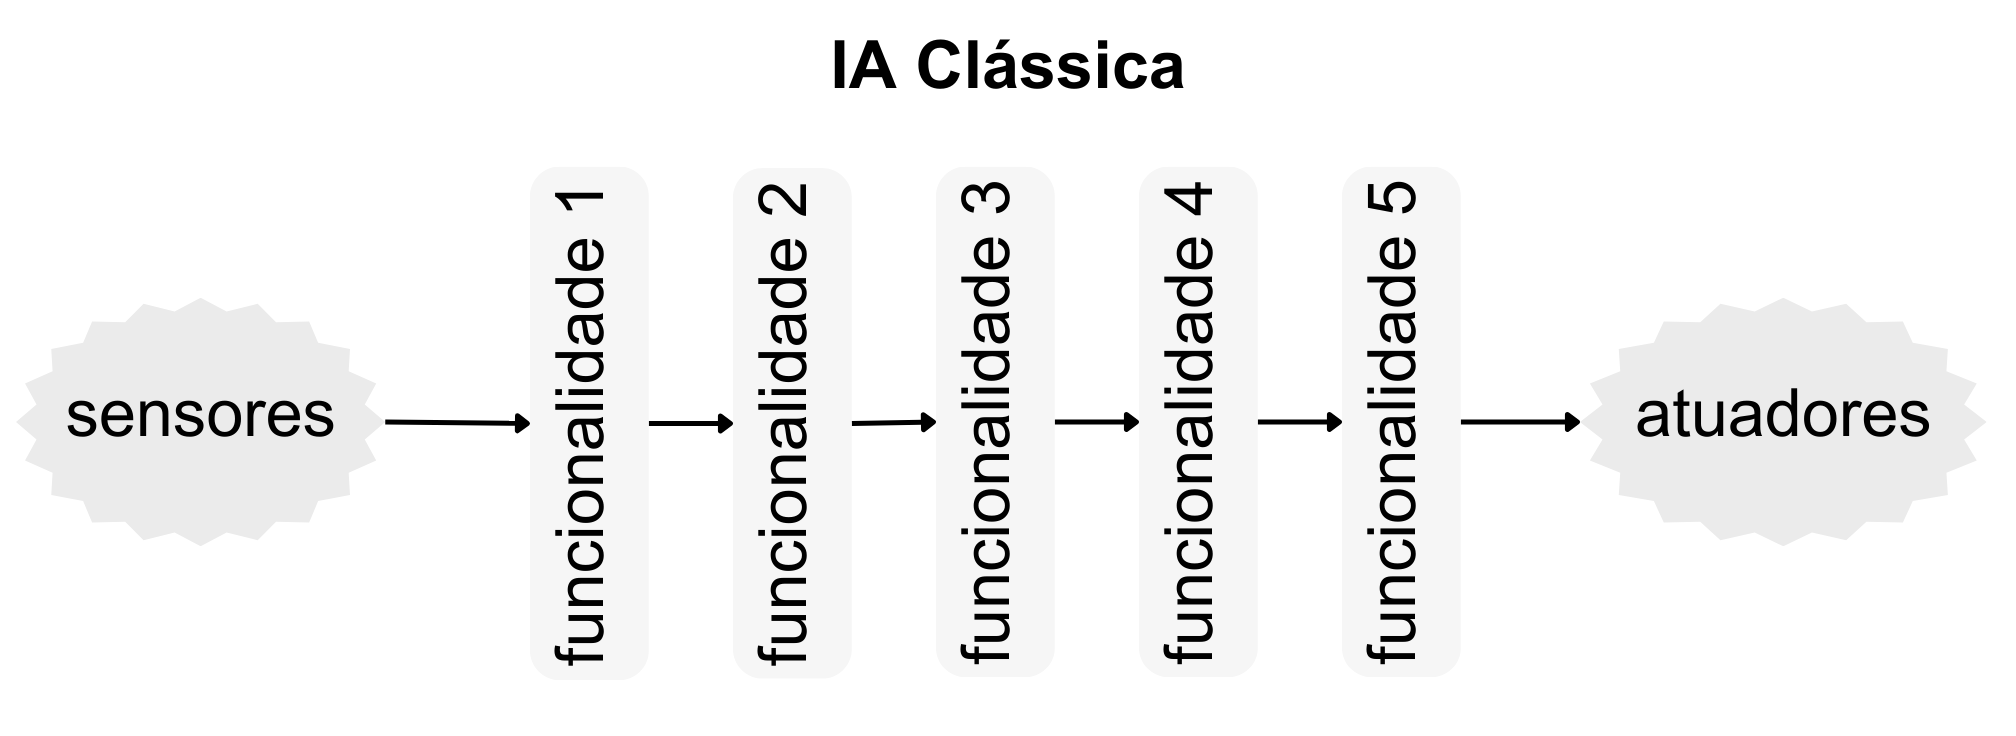
\includegraphics[scale=0.3]{iaclassica.png}
    \caption*{Fonte: Adaptação de \citet{brooks85} pela autora.}
    \label{fig:iaclassica}
\end{figure}

Como visto, a abordagem hierarquica cria uma dependência entre suas funcionalidades. Essa característica permite a diminuição da robustez do sistema, já que o erro em uma das suas funcionalidades resulta em uma falha generalizada \cite{practicalIndroductionNehmzow:2012}. Além disso, as camadas mais centrais se baseiam unicamente em modelos do mundo real e dos resultados de processamento antecessores, causando uma menor confiabilidade no sistema e reflexos mais lentos à dinamicidade do ambiente \cite{practicalIndroductionNehmzow:2012}.

As abordagens comportamentais, introduzidas pela arquitetura de subsunção, têm o intuito de controlar o robô por comportamentos independentes e assíncronos, ativados conforme os acontecimentos do ambiente, sendo sistemas reativos \cite{seqlam:2020, toroco:2022}. Como exposto na Figura~\ref{fig:subsuncao}, o controle lógico do robô é dividido em funcionalidades que representam comportamentos distintos e são executadas paralelamente. Todas as funcionalidades são alimentadas com os dados captados dos sensores e inferem comandos nos atuadores \cite{seqlam:2020,brooks85}. Logo, o conjunto da execução de todas as funcionalidades resulta na atuação do objetivo final do robô.

\begin{figure}[h]
    \centering
    \caption{Arquitetura de subsunção}
    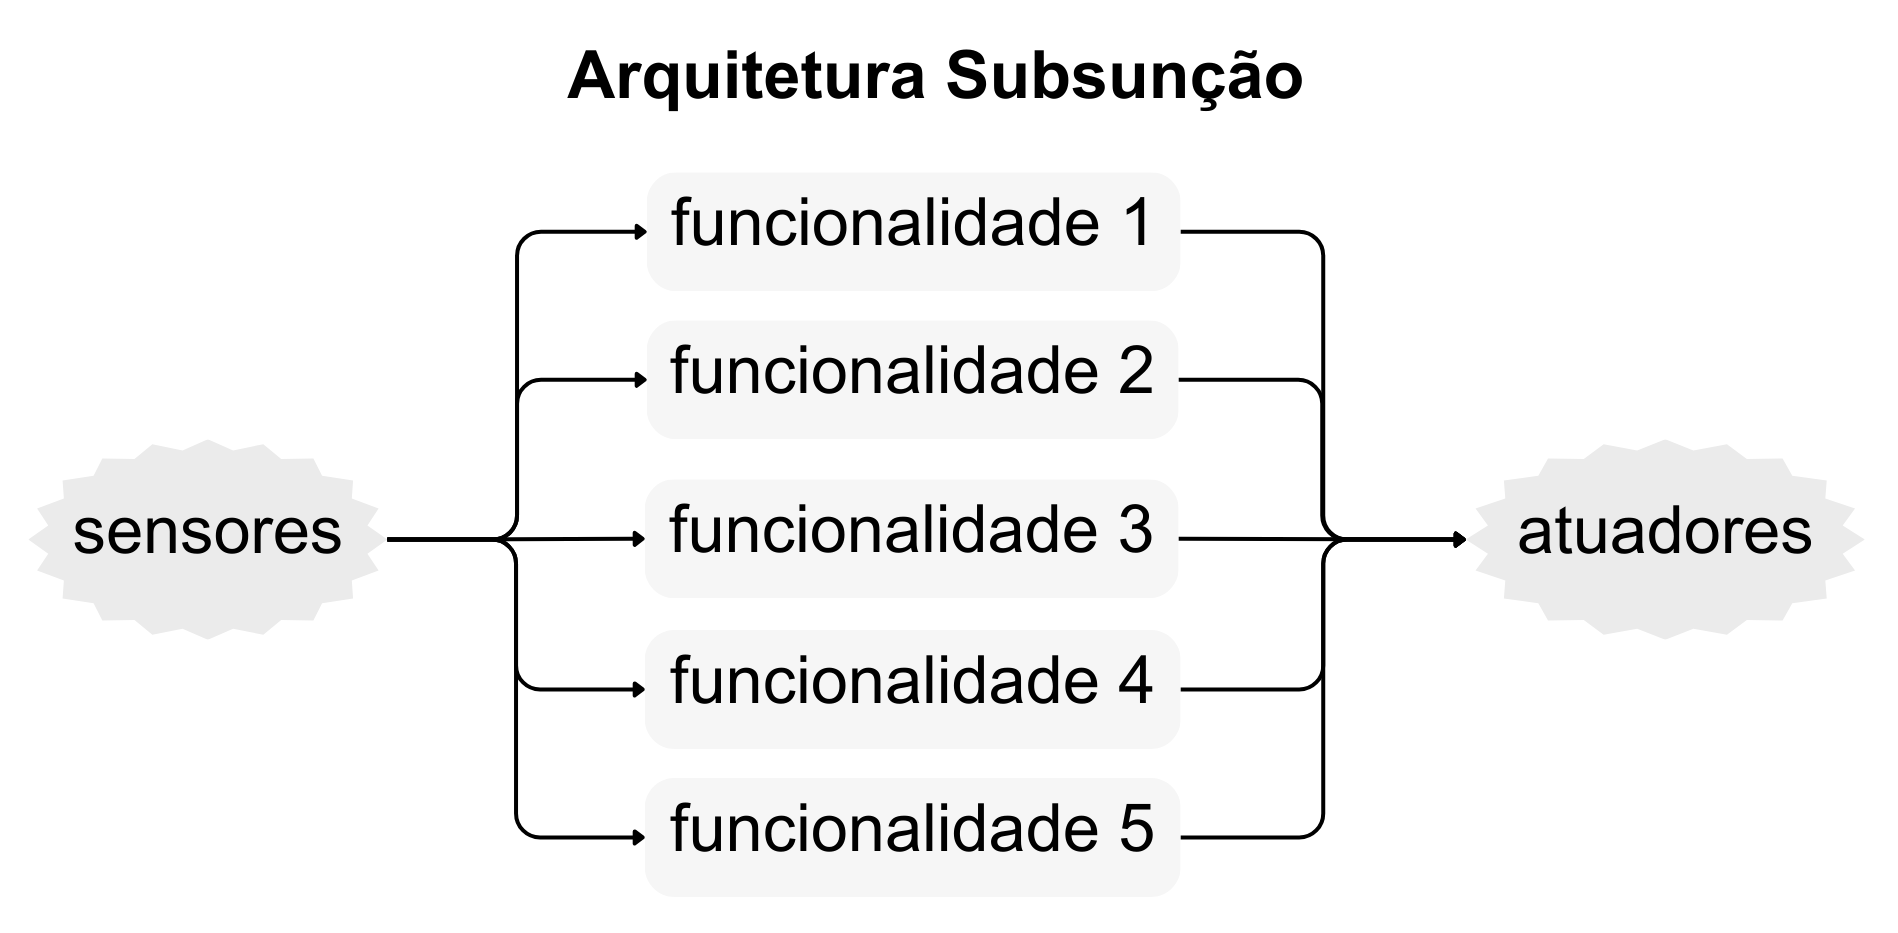
\includegraphics[scale=0.4]{subsuncao.png}
    \caption*{Fonte: Adaptação de \citet{brooks85} pela autora.}
    \label{fig:subsuncao}
\end{figure}

As características das abordagens comportamentais permitem algumas vantagens em comparação com as abordagens hierarquicas. Entre essas vantagens, se destacam i) a redução do custo computacional; ii) a maior confiabilidade por conta do acesso direto às informações do ambiente por cada camada; iii) a maior robustez causada pela independência das camadas \cite{seqlam:2020,brooks85, toroco:2022}. 

As camadas da arquitetura de subsunção foram projetadas por \citet{brooks85} como níveis de competência que especificam, informalmente, uma classe de comportamentos desejáveis. Neste trabalho, Brooks utilizou cinco níveis que contemplam navegação, com e sem rumo, evitando colisões, exploração e mapeamento do ambiente, planejamento de rotas e tratamento de mudanças no espaço. Entretanto, a independência entre cada camada da arquitetura permite o incremento, ou remoção, de funcionalidades conforme o cenário de atuação do robô. 

\citet{brooks85} expõe nove paradigmas para os sistemas baseados na arquitetura proposta. Entre eles, salienta-se a importância da simplicidade em diversos aspectos, como o próprio sistema de controle a ser implementado e a comunicação entre as camadas. 

Outra questão levantada na arquitetura de subsunção é o uso de modelos do mundo (tais quais não são usados unicamente durante o processamento, pois todos os módulos têm acesso às informações coletadas pelos sensores). Eles visam uma melhor verossimilidade a realidade a partir do uso de mapas não relacionais de três dimensões e não artificiais. Por fim, também é ressaltado a necessidade da durabilidade e robustez do sistema sem a interferência de humanos.


\subsection{Estrutura Física do Robô} 

A estrutura física do robô precisa refletir e acomodar o ambiente em que atua para as suas tarefas serem executadas correta e eficientemente. O corpo, que engloba o sistema implementado, pode consistir em sensores que irão coletar dados do ambiente e da condição do próprio dispositivo, atuadores para terem ações sobre o meio, partes mecânicas como braços robóticos para manipulações e elementos para o processamento geral e individual dos outros componentes.

A percepção do ambiente e a execução das tarefas pelo robô dependem significativamente dos transdutores para tais fins, disponibilizados no seu corpo. Como \citet{instrumentacao:2013} explica, os transdutores são dispositivos utilizados para captarem dados (grandezas físicas)  do ambiente e transformarem em informações (sinais elétricos) para o sistema processar ou transformarem decisões tomadas (sinais elétricos) pelo processamento do sistema em ações (grandezas físicas) executadas no ambiente. Assim, existem dois tipos de transdutores: os sensores e os atuadores. 

Os sensores são responsáveis em permitir que o robô compreenda o ambiente que está inserido através das grandezas físicas coletadas (entradas) e transformadas em sinais elétricos que então são processados em uma informação útil (saída). Apesar de comumente os sensores obterem entradas que não são as em foco (entradas espúrias), são utilizados diversos mecanismos de filtrar entradas e calibrar estes instrumentos para seu melhor desempenho. 

O mundo dos sensores  é versátil e variado, dentre os existentes para a percepção de objetos se tem o sensor LiDaR (\textit{Light Detection and Ranging}), o qual emite uma onda ótica e captura o tempo para que o reflexo desse feixe de luz retorne \cite{lidarComparative:2021, lidarProgress:2022}. Seu objetivo principal é descobrir a distância entre o corpo que está embutido e os objetos à sua frente \cite{lidarProgress:2022, lidarComparative:2021}. Esse sensor é utilizado em diversas situações, como veículos autônomos, equipamentos médicos precisos e monitoramento, podendo ser mais preciso do que sensores que utilizam ondas sonoras \cite{lidarProgress:2022, lidarDetection:2019}.

Os atuadores, por sua vez, possibilitam que as tarefas planejadas pelo sistema se concretizem a partir do inferimento de grandezas físicas em elementos mecânicos presentes no corpo do robô. Este comportamento pode ser visualizado quando o controle lógico de um robô móvel autônomo decide se virar para direita e pelos atuadores, os motores necessários são acionados para realizar a rotação das rodas.  

A arquitetura de subsunção apresentada por \citet{brooks85} também trata sobre questões do corpo físico do robô. Em primeiro lugar é retratado que o dispositivo deve possuir uma estrutura que o permite trafegar em espaços de convivência de humanos, isso implica que ele deve ter uma certa altura para conseguir enxergar objetos em cima de móveis, por exemplo, e uma largura máxima para conseguir passar por portas e corredores. 

Em \citet{brooks85}, também é reforçada a importância da independência dos sensores e outros instrumentos de percepção, trazendo maior robustez ao sistema e confiabilidade, mesmo se alguns de seus sensores apresentarem erro. 

\section{Simulação} %%ATUALIZADO

A construção de um robô e o teste da sua estrutura em conjunto com o software de controle requerem um leque grande de recursos e bastante tempo disponível. Por isso, quando há uma escassez, limitações ou nenhuma disponibilidade de algum desses requisitos, podem ser usados simuladores que representam e interpretam o mundo real virtualmente. 
Tais ferramentas são utilizadas em diversos campos das engenharias, inclusive a robótica, sendo muito prático para pesquisa e educação \cite{usarsimCarpin:2007}. 

Como o intuito dos experimentos virtuais consiste em simular eventos reais que poderiam existir em testes no mundo tangível, é preciso ter cautela e incluir a maior veracidade possível ao ambiente e robô simulados \cite{aprendizadoHeinen:2010}.  
Assim, se faz necessário a modelagem de leis da física presentes no universo real e a interação com ambiente por sensores e atuadores, para o robô sofrer quedas e colisões segundo a situação, conforme a realidade \cite{usarsimCarpin:2007, evolucaoHeinen:2006}.  

A maior preocupação acerca do uso da simulação é a sua capacidade de conter detalhes verídicos e ser o menos limitante possível, visto que o mundo  real é muito mais complexo  \cite{wanderingMiglino:1994}. 
Com um experimento por \citet{wanderingMiglino:1994} para o teste de algoritmos que propõem a evolução de robôs vagantes, foi demonstrado que a simulação e a execução real desses robôs conseguem ser bem similares, obtendo melhor desempenho em robôs tangíveis para alguns casos.

Os simuladores permitem interpretar situações reais de forma virtual. Entretanto, é necessário intermediar os elementos (sensores e atuadores) do robô com seu controle lógico. Isso é possível ao implementar ROS (Sistema Operacional de Robô), o kit de desenvolvimento para aplicações robóticas \cite{ROS} Uma das maiores vantagens do ROS é a sua coleção de bibliotecas e módulos para utilizar em diversas ocasiões robóticas, sem a necessidade de desenvolver algoritmos do início \cite{ROS}. Além disso, ROS é multi-plataforma, possibilitando o desenvolvimento único  para a simulação e a realidade \cite{ROS}.

Para reconstruir virtualmente os elementos reais, é necessário descrever, em XML (\textit{eXtensible Markup Language}), as suas características físicas, dinâmicas, cinemáticas e o comportamento das suas ações \cite{geradorURDF:2019, geradorURDF:2022, sdf:2019}. Esta descrição pode ser realizada de diversas maneiras, como no formato universal (URDF - \textit{Universal Robotic Description Format}), permitindo amplo reconhecimento pela maioria dos simuladores com integração do ROS, ou no formato padrão de descrição (SDF - \textit{Standard Description Format}), com o intuito de caracterizar o conjunto do meio de atuação do robô além de seus próprios atributos \cite{geradorURDF:2019, geradorURDF:2022, sdf:2019}.

Nesse contexto de programas de simulação robótica,  é possível encontrar desde ambientes gratuitos mais rústicos para pesquisa e educação, como USARSim,  até os mais profissionais oferecidos por empresas especializadas em desenvolvimento de eletrônicos, como a Nvidia que oferece o Nvidia Omniverse e a biblioteca IsaacSim para simulação de robótica. 

Também é possível encontrar soluções no meio-termo que são muito utilizadas como WeBot da Cyberbotics, Gazebo e CoppeliaSim, tais quais são \textit{open source} e utilizam a biblioteca Open Dynamics Engine (ODE) para trazer aspectos da física na simulação.  A ODE também pode ser integrada em plataformas de criação de jogos, como a Unity, transformando-as em ambientes simuladores de robótica. 

Dentre os supracitados, pode ser destacado o simulador \textit{open-source} Gazebo \cite{gazeboDesigns:2004}. Algumas de suas características que o faz ser ressaltado em meio aos diversos outros simuladores são: i) modelos de robôs e ambientes prontos; ii) comunidade ativa que visa incrementar novos modelos de robôs e ambientes; iii) integração com ROS \cite{gazeboDesigns:2004, pickSimulatorFarley:2022}.

\section{Considerações Adicionais da Fundamentação Teórica}

Este capítulo permitiu uma fundamentação teórica nos principais tópicos dos robôs autônomos móveis e a simulação robótica. Foram discutidos os quatro aspectos da navegação autônoma de um robô que consiste na percepção do ambiente, sua localização, o planejamento de uma rota a ser seguida e a sua locomoção. 

Além disso, foi compreendida a arquitetura de subsunção para o controle do robô e a sua vantagem com relação à abordagem tradicional da inteligência artificial. Ainda no contexto dos robôs, foram introduzidas as necessidades para a sua estrutura física.  Por fim, foi explorado o tema de simulação robótica, alguns programas simuladores reconhecidos e o sistema operacional de robô. 

Com essa compreensão do funcionamento de robôs autônomos móveis e da simulação robótica, se torna possível analisar mais vigorosamente trabalhos que almejam desenvolver um robô com a capacidade de navegar de forma autônoma em um ambiente interno desconhecido. Assim, o próximo capítulo expõe variados trabalhos correlatos, além das suas diferenças e similaridades com o AtmosBot.


